\section{Bewijslast}
Dit hoofdstuk bevat de bewijslast voor de leerdoelen die in het Plan van Aanpak staan. Hier zal een apart hoofdstuk per leerdoel komen waar in diepte wordt uitgelegd waarom dit leerdoel is behaald.

\subsection{Professioneel functioneren}
Op 25 november 2014 is mijn stagedocent langs gekomen. Toen heeft mijn stagebegeleider een evaluatie over mij ingevuld waarmee ik word beoordeeld op het professionele functioneren. Het eerste STARTT formulier hier onder zal gaan over deze evaluatie. Daarin wordt gereflecteerd op

\newline
Mijn stagebegeleider heeft aan het einde van mijn stageperiode een eindbeoordeling ingevuld, ook hier is op gereflecteerd in de vorm van een STARRT formulier. Het tweede STARRT formulier hier onder zal gaan over deze eindbeoordeling.

\subsubsection{STARRT Formulieren}

\textbf{STARRT Formulier 1: Tussenbeoordeling}

\begin{tabularx}{\textwidth}{| l | X |}
\hline
\multicolumn{2}{|l|}{Academie: Academie voor Technologie \& Innovatie } \\
\hline
\multicolumn{2}{|l|}{Opleiding: HBO-ICT } \\
\hline
\multicolumn{2}{|l|}{Studentnaam: Joey Kaan \hspace{35pt} Studentnummer: 64808} \\
\hline
\multicolumn{2}{|l|}{Stagedocent: D. de Waard} \\
\hline
\multicolumn{2}{|p{\textwidth-1in}|}{Leerdoel/competentie: Professioneel functioneren.} \\
\hline
\multicolumn{2}{|l|}{Cursus: Meewerkstage \hspace{35pt} Cursuscode: CU06322} \\
\hline
\multicolumn{2}{|l|}{Datum: \today} \\
\hline
\multicolumn{2}{|l|}{
\begin{minipage}{0.9\columnwidth}
Titel en nummer van bewijs/bewijzen:
\begin{itemize}
\item Bewijs 2: Tussenbeoordeling
\end{itemize}
\end{minipage}
} \\ [50pt]
\hline
\multicolumn{2}{|l|}{Oordeel: } \\
\hline
S & Geef voorbeelden van opdrachten (situaties) waarmee je kunt aantonen dat je de competentie hebt verworven. Beschrijf kort wat er aan de hand was of om welke opdracht het ging.
\newline
\newline
De opdracht was professioneel functioneren. Ik heb bij Connect Social Business 105 dagen stage moeten lopen. Tijdens deze stage periode wordt er op een professionele manier gewerkt, dat wordt bedoeld met het professionele functioneren.
\\
\hline
T & Beschrijf de exacte rol/taak die jij had. Geef aan of het om een complexe taak ging en waaruit dat bleek. Wat moest jij doen?
\newline
\newline
Ik heb stage gelopen bij Connect Social Business als een web developer. Ik heb Content2Connect gewerkt waar alleen ik aan heb gewerkt dus waarbij ik niet hoefde te overleggen met iemand, alleen als er bijvoorbeeld een release uitgebracht moest worden dan moest ik dit overleggen met Kevin, dat is de lead developer. Naast Content2Connect heb ik ook aan Profile2Connect gewerkt. Dit project wordt samen gedaan met 2 andere mensen en hierbij moest er dus heel veel overlegd worden. Hoe het beste de architectuur van het platform opgezet kon worden, wat voor design patterns we gebruiken en wat voor algoritmes we gebruiken om bepaalde zaken op te lossen. Dat zijn een aantal voorbeelden van vragen die gesteld worden en waar over gediscussierd wordt.
\\
\hline
A & Beschrijf de activiteiten die jij achtereenvolgens hebt ondernomen in het kader van deze opdracht. Wat heb je concreet gedaan?
\newline
\newline
Tijdens het stage lopen heb ik natuurlijk een groot aantal aan activiteiten moeten doen. Een opsomming van deze activiteiten bevindt zich hieronder. Deze zullen verdeeld zijn over de opdrachten die mij toegewezen waren tijdens mijn stage periode; Content2Connect en Profile2Connect.

Voor Content2Connect:
\begin{itemize}
\item Functioneel ontwerp maken Content2Connect; gesprek met opdrachtgever (Paul)
\item Nadenken over technische architectuur Content2Connect
\item Uitwerken prototype Content2Connect
\item Uitwerking prototype bespreken met lead developer (Kevin)
\item Feedback verwerken van lead developer
\item Uitwerking prototype bespreken met opdrachtgever (Paul)
\item Feedback verwerken van opdrachtgever
\item Daadwerkelijk Content2Connect gaan ontwerpen \& programmeren
\item Tests schrijven voor Content2Connect
\end{itemize}

Voor Profile2Connect:
\begin{itemize}
\item Samen met andere twee collega's structuur bespreken van Profile2Connect
\item Functionaliteit duidelijk krijgen voor Profile2Connect; gesprek met opdrachtgever (Jeroen)
\item Uitwerken functionaliteit in prototype
\item Klaarmaken voor release; tests schrijven en afronden development
\item Functionaliteit volgende release duidelijk krijgen voor Profile2Connect; gesprek met opdrachtgever (Jeroen)
\end{itemize}
\\
\hline
R & Beschrijf het resultaat van de opdracht en hoe de betrokkenen er op reageerden. Wat is er vervolgens met dat resultaat gebeurd?
\newline
\newline
Alhoewel bij de activiteiten concrete opdrachten worden beschreven is het resultaat van dit leerdoel niet zozeer iets fysieks. Het is meer een gevoel dat mensen bij de persoon hebben en op basis van dit gevoel kunnen ze een evaluatie invullen.
Kevin, de lead developer, heeft dus een evaluatie ingevuld met zijn mening over hoe ik tijdens mijn stage professioneel heb gefunctioneerd. De evaluatie is te zien in de bijlage.
\\
\hline
R & Wat heb je ervan geleerd? Wat zou je volgende keer anders aanpakken en waarom?
\newline
\newline
Uit de evaluatie blijkt dat ik op eigenlijk alle punten boven het gemiddelde zit, alleen bij nauwkeurigheid en stiptheid ben ik gemiddeld. Hoewel ik natuurlijk aan alle punten zal blijven werken heb ik wel geleerd dat ik nauwkeuriger en stipter moet gaan werken, dit is natuurlijk een zeer belangrijke kwaliteit van een developer.
\newline
Wat betreft mijn mening over de evaluatie, ik vind dat mijn stagebegeleider mij heel goed heeft ingeschat. Ik heb vaak moeite met het nauwkeurig werken omdat ik altijd die druk voel dat het snel af moet komen. Vaak is de oplossing die even snel bedacht wordt wel functioneel maar niet zozeer de beste oplossing. Ik denk dat ik wat vaker naar mijn gemaakte code zou moeten kijken op zoek naar dingen die verbeterd kunnen worden. Als ik mijn nulmeting met het evaluatieformulier ingevuld door mijn stagebegeleider vergelijk is te zien dat ik mijzelf niet heel optimistisch beoordeelde, maar dat mijn negatieve houding niet nodig was.. De actiepunten die ik hiervan kan halen is dat ik nauwkeuriger ga werken, wat meer tijd nemen om een goede oplossing te bedenken en nadat ik de oplossing heb geprogrammeerd nog eens goed kijken of het toch niet beter kan.
\\
\hline
T & Geef een voorbeeld van een andere situatie waarin je deze competentie kunt toepassen
\newline
\newline
Deze competentie is natuurlijk te gebruiken bij elke situatie in het bedrijfsleven. Het moet altijd prioriteit hebben dat je professioneel omgaat met collega's en opdrachtgevers. Ik weet nu waar mijn plus punten zijn en waar mijn min punten liggen, omdat ik deze nu weet kan ik deze van te voren aangeven aan mijn collega's zodat ze op de hoogte zijn van eventuele tekortkomingen die ik kan vertonen. Zo weten ze ook wat ze van mij kunnen verwachten en is het ook makkelijker in te schatten hoeveel tijd een bepaald project zal kosten.
\\
\hline
\end{tabularx}

\clearpage

\textbf{STARRT Formulier 2: Eindbeoordling}

\begin{tabularx}{\textwidth}{| l | X |}
\hline
\multicolumn{2}{|l|}{Academie: Academie voor Technologie \& Innovatie } \\
\hline
\multicolumn{2}{|l|}{Opleiding: HBO-ICT } \\
\hline
\multicolumn{2}{|l|}{Studentnaam: Joey Kaan \hspace{35pt} Studentnummer: 64808} \\
\hline
\multicolumn{2}{|l|}{Stagedocent: D. de Waard} \\
\hline
\multicolumn{2}{|p{\textwidth-1in}|}{Leerdoel/competentie: Professioneel functioneren (Eindbeoordeling)} \\
\hline
\multicolumn{2}{|l|}{Cursus: Meewerkstage \hspace{35pt} Cursuscode: CU06322} \\
\hline
\multicolumn{2}{|l|}{Datum: \today} \\
\hline
\multicolumn{2}{|l|}{
\begin{minipage}{0.9\columnwidth}
Titel en nummer van bewijs/bewijzen:
\begin{itemize}
\item Bewijs 3: Eindbeoordeling
\end{itemize}
\end{minipage}
} \\ [50pt]
\hline
\multicolumn{2}{|l|}{Oordeel: } \\
\hline
S & Geef voorbeelden van opdrachten (situaties) waarmee je kunt aantonen dat je de competentie hebt verworven. Beschrijf kort wat er aan de hand was of om welke opdracht het ging.
\newline
\newline
De opdracht was professioneel functioneren. Ik heb bij Connect Social Business 105 dagen stage moeten lopen. Tijdens deze stage periode wordt er op een professionele manier gewerkt, dat wordt bedoeld met het professionele functioneren.
\\
\hline
T & Beschrijf de exacte rol/taak die jij had. Geef aan of het om een complexe taak ging en waaruit dat bleek. Wat moest jij doen?
\newline
\newline
Ik heb stage gelopen bij Connect Social Business als een web developer. Ik heb Content2Connect gewerkt waar alleen ik aan heb gewerkt dus waarbij ik niet hoefde te overleggen met iemand, alleen als er bijvoorbeeld een release uitgebracht moest worden dan moest ik dit overleggen met Kevin, dat is de lead developer. Naast Content2Connect heb ik ook aan Profile2Connect gewerkt. Dit project wordt samen gedaan met 2 andere mensen en hierbij moest er dus heel veel overlegd worden. Hoe het beste de architectuur van het platform opgezet kon worden, wat voor design patterns we gebruiken en wat voor algoritmes we gebruiken om bepaalde zaken op te lossen. Dat zijn een aantal voorbeelden van vragen die gesteld worden en waar over gediscussierd wordt.
\\
\hline
A & Beschrijf de activiteiten die jij achtereenvolgens hebt ondernomen in het kader van deze opdracht. Wat heb je concreet gedaan?
\newline
\newline
Tijdens het stage lopen heb ik natuurlijk een groot aantal aan activiteiten moeten doen. Een opsomming van deze activiteiten bevindt zich hieronder. Deze zullen verdeeld zijn over de opdrachten die mij toegewezen waren tijdens mijn stage periode; Content2Connect en Profile2Connect.

Voor Content2Connect:
\begin{itemize}
\item Functioneel ontwerp maken Content2Connect; gesprek met opdrachtgever (Paul)
\item Nadenken over technische architectuur Content2Connect
\item Uitwerken prototype Content2Connect
\item Uitwerking prototype bespreken met lead developer (Kevin)
\item Feedback verwerken van lead developer
\item Uitwerking prototype bespreken met opdrachtgever (Paul)
\item Feedback verwerken van opdrachtgever
\item Daadwerkelijk Content2Connect gaan ontwerpen \& programmeren
\item Tests schrijven voor Content2Connect
\end{itemize}

Voor Profile2Connect:
\begin{itemize}
\item Samen met andere twee collega's structuur bespreken van Profile2Connect
\item Functionaliteit duidelijk krijgen voor Profile2Connect; gesprek met opdrachtgever (Jeroen)
\item Uitwerken functionaliteit in prototype
\item Klaarmaken voor release; tests schrijven en afronden development
\item Functionaliteit volgende release duidelijk krijgen voor Profile2Connect; gesprek met opdrachtgever (Jeroen)
\end{itemize}
\\
\hline
R & Beschrijf het resultaat van de opdracht en hoe de betrokkenen er op reageerden. Wat is er vervolgens met dat resultaat gebeurd?
\newline
\newline
Alhoewel bij de activiteiten concrete opdrachten worden beschreven is het resultaat van dit leerdoel niet zozeer iets fysieks. Het is meer een gevoel dat mensen bij de persoon hebben en op basis van dit gevoel kunnen ze een evaluatie invullen.
Kevin, de lead developer, heeft dus een evaluatie ingevuld met zijn mening over hoe ik tijdens mijn stage professioneel heb gefunctioneerd. De evaluatie is te zien in de bijlage.
\\
\hline
R & Wat heb je ervan geleerd? Wat zou je volgende keer anders aanpakken en waarom?
\newline
\newline
Aan de hand van de eindbeoordeling kan ik afleiden dat ik ten opzichte van mijn tussenbeoordeling zeker vorderingen heb gemaakt. Ik heb na de tussenbeoordeling gelet op het nauwkeuriger en stipter werken en aan de hand van de eindbeoordeling is ook te zien dat dit een positief effect heeft gehad. De conclusie die ik hier uit kan trekken is dat ik gewoon door moet gaan met hoe ik nu al doe. Het beste is om wel nog steeds te letten op het nauwkeurige werken, want dat is denk ik een zwak puntje van mij.
\\
\hline
T & Geef een voorbeeld van een andere situatie waarin je deze competentie kunt toepassen
\newline
\newline
Deze competentie is natuurlijk te gebruiken bij elke situatie in het bedrijfsleven. Het moet altijd prioriteit hebben dat je professioneel omgaat met collega's en opdrachtgevers. Ik weet nu waar mijn plus punten zijn en waar mijn min punten zijn, omdat ik deze nu weet kan ik deze van te voren aangeven aan mijn collega's zodat ze op de hoogte zijn van eventuele tekortkomingen die ik kan vertonen. Zo weten ze ook wat ze van mij kunnen verwachten en is het ook makkelijker in te schatten hoeveel tijd een bepaald project zal kosten.
\\
\hline
\end{tabularx}

\subsubsection{Bewijzen}
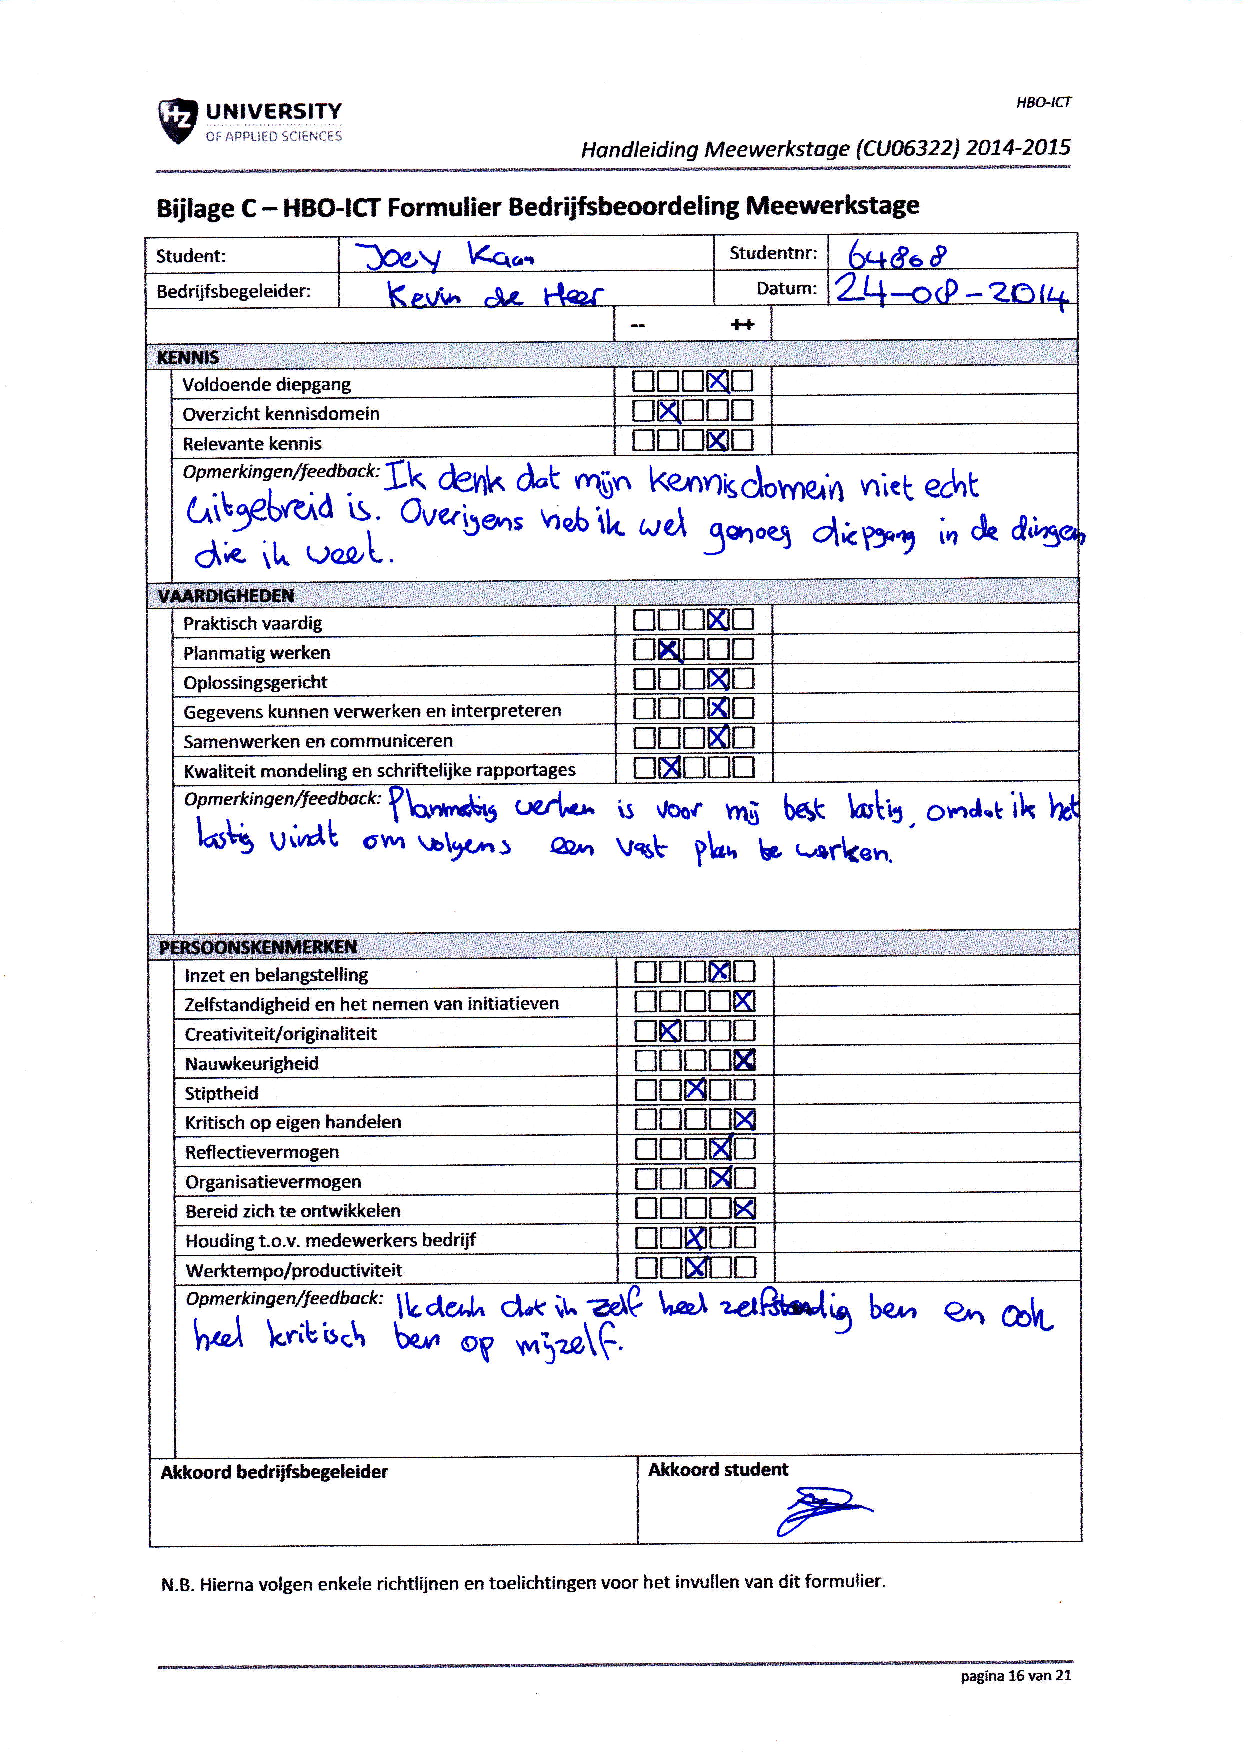
\includepdf[pages={1}, scale=0.65, pagecommand=\textbf{Bewijs 1: Nulmeting}\thispagestyle{fancy}]{attachments/Nulmeting.pdf}
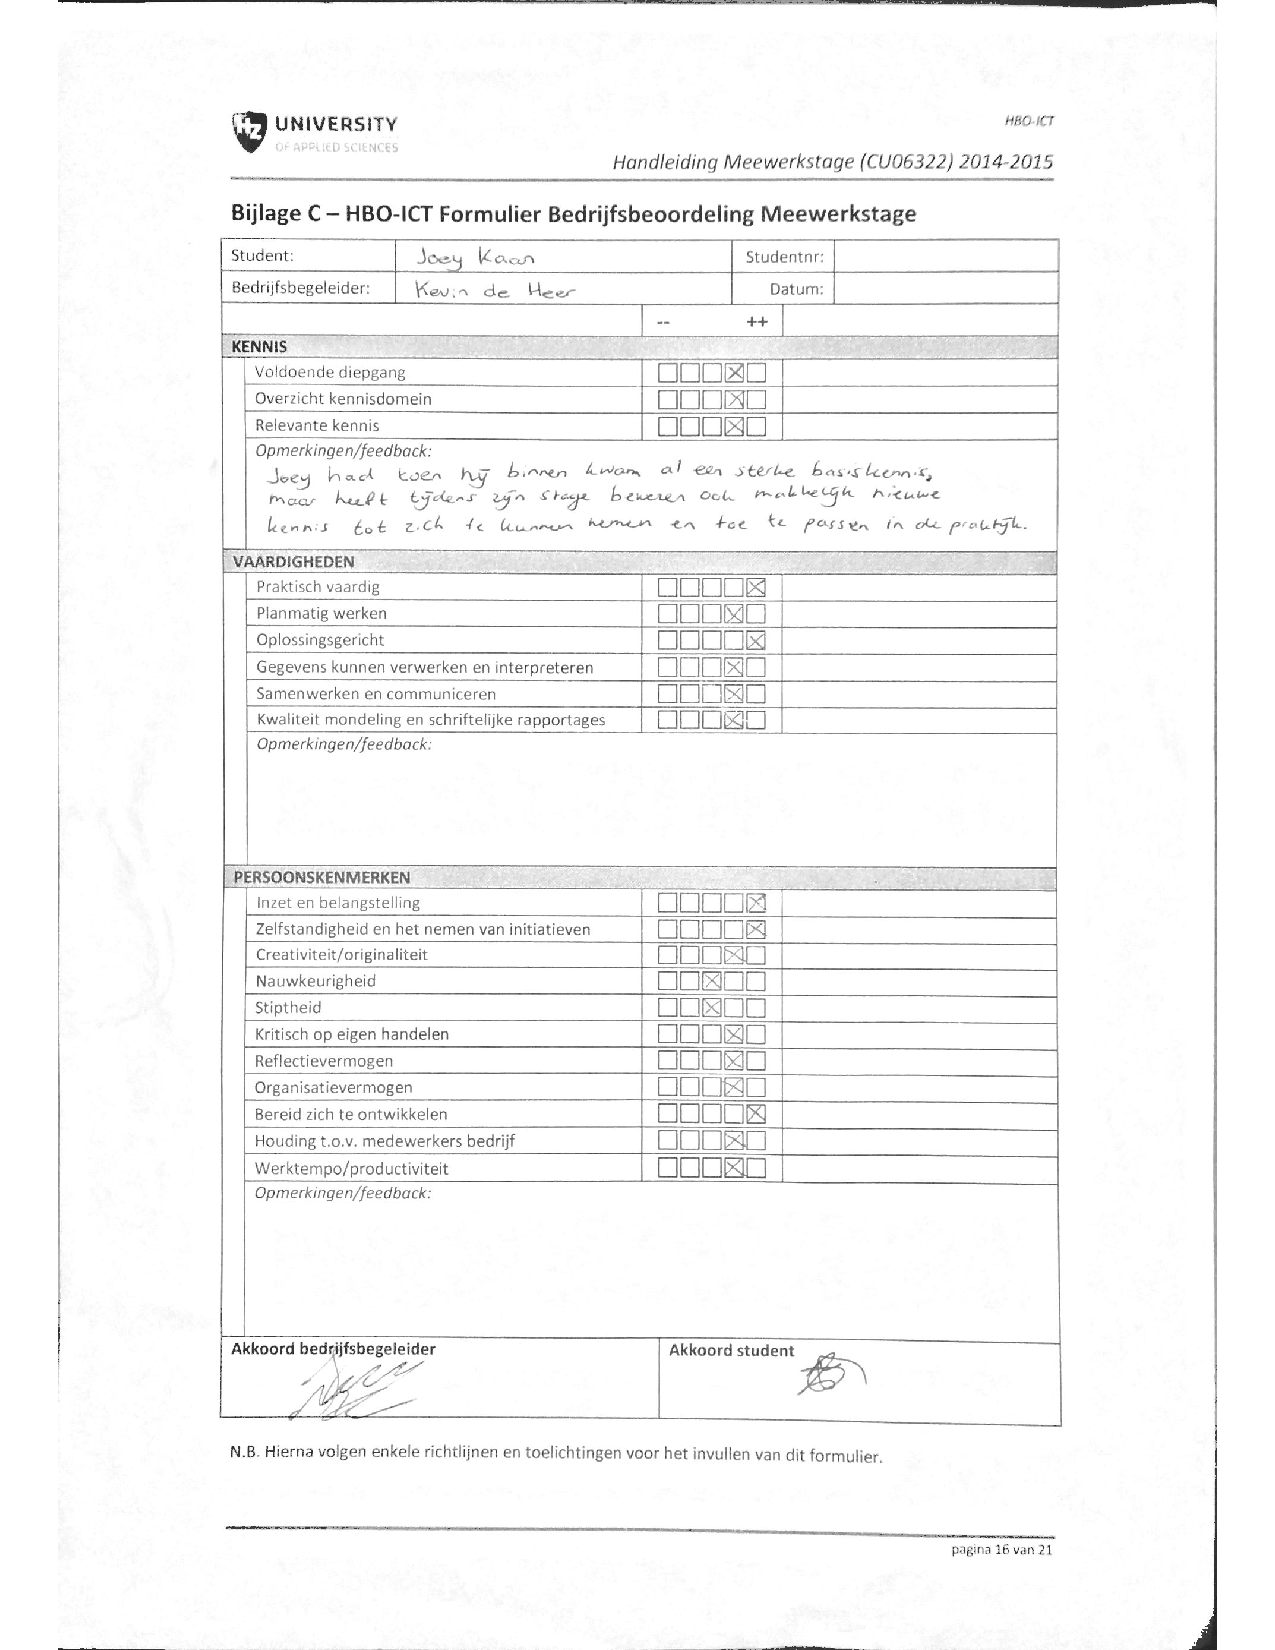
\includepdf[pages={1}, scale=0.65, pagecommand=\textbf{Bewijs 2: Tussenbeoordling}\thispagestyle{fancy}]{attachments/tussenbeoordeling.pdf}
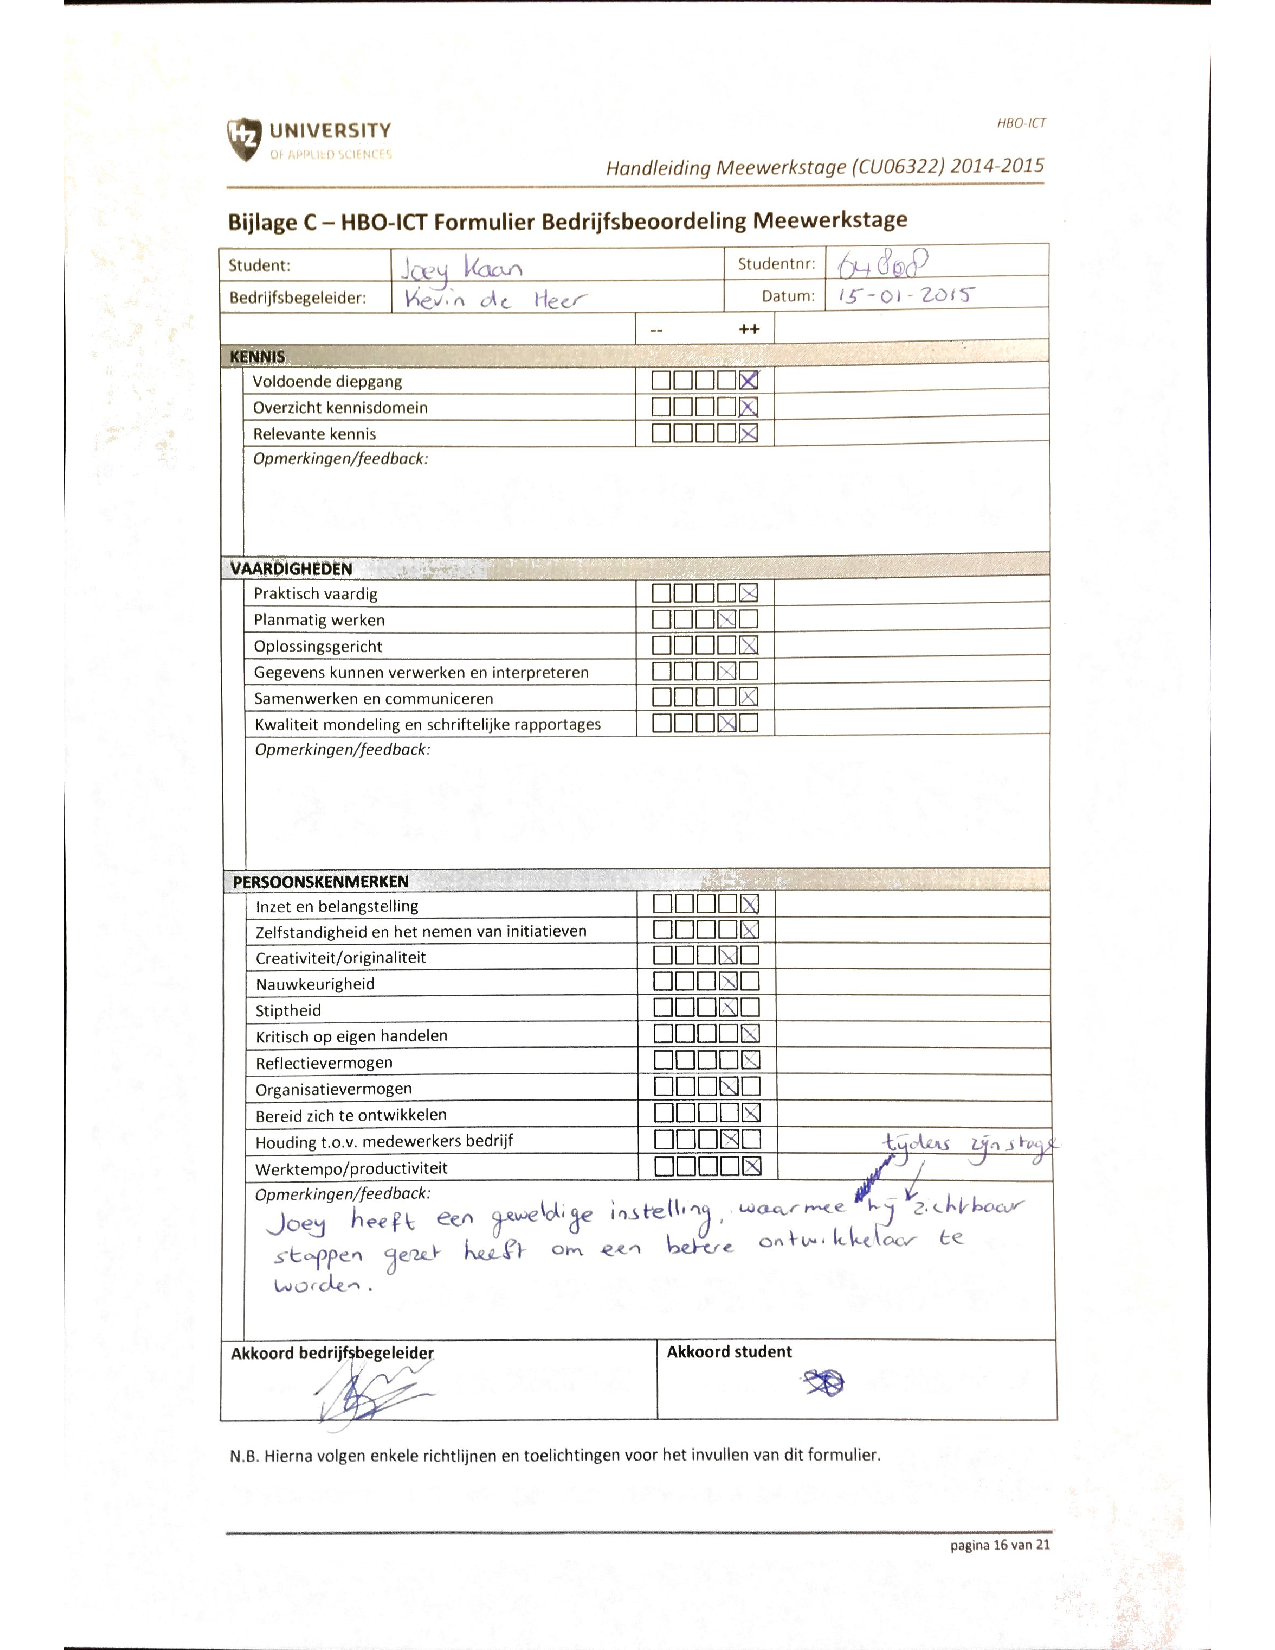
\includepdf[pages={1}, scale=0.65, pagecommand=\textbf{Bewijs 3: Eindbeoordeling}\thispagestyle{fancy}]{attachments/eindbeoordeling.pdf}

\subsection{Facebook API}
Het volledige leerdoel dat ook beschreven staat in het Plan van Aanpak gaat als volgt: Facebook API leren door middel van een applicatie te maken die hiervan gebruik maakt door informatie van een pagina van een klant op te halen. Overigens ben ik mijn hele stage periode bezig geweest aan Content2Connect en Profile2Connect dus hiernaast nog een aparte applicatie maken die gebruik maakte van de Facebook API zat er niet bij. Profile2Connect had overigens wel een aantal zaken moeten doen met de Facebook API en hier heb ik dus dit leerdoel nu op gebaseerd.

\subsubsection{STARRT Formulier}
\begin{tabularx}{\textwidth}{| l | X |}
\hline
\multicolumn{2}{|l|}{Academie: Academie voor Technologie \& Innovatie } \\
\hline
\multicolumn{2}{|l|}{Opleiding: HBO-ICT } \\
\hline
\multicolumn{2}{|l|}{Studentnaam: Joey Kaan \hspace{35pt} Studentnummer: 64808} \\
\hline
\multicolumn{2}{|l|}{Stagedocent: D. de Waard} \\
\hline
\multicolumn{2}{|p{\textwidth-1in}|}{Leerdoel/competentie: Facebook API leren door middel van een applicatie te maken die hiervan gebruik maakt door informatie van een pagina van een klant op te halen.} \\
\hline
\multicolumn{2}{|l|}{Cursus: Meewerkstage \hspace{35pt} Cursuscode: CU06322} \\
\hline
\multicolumn{2}{|l|}{Datum: \today} \\
\hline
\multicolumn{2}{|l|}{
\begin{minipage}{0.9\columnwidth}
Titel en nummer van bewijs/bewijzen:
\begin{itemize}
\item Bewijs 1: Beoordelingsformulier
\item Bewijs 2: Uitwerking
\end{itemize}
\end{minipage}
} \\ [50pt]
\hline
\multicolumn{2}{|l|}{Oordeel: } \\
\hline
S & Geef voorbeelden van opdrachten (situaties) waarmee je kunt aantonen dat je de competentie hebt verworven. Beschrijf kort wat er aan de hand was of om welke opdracht het ging.
\newline
\newline
Tijdens het ontwikkelen van Profile2Connect wordt er al vanaf een ander platform data van Facebook meegestuurd. Profile2Connect is gebaseerd op profielen en de data die mee wordt gestuurd zijn alleen maar ID's van mensen op Facebook. Zo moet Profile2Connect dus nog zelf informatie van de Facebook API ophalen van alle ID's die binnenkomen. De opdracht was dus om van die ID's een logische lijst te maken die dan opgestuurd kon worden naar de Facebook API. Als dit dan gelukt was, was het daarna de bedoeling om de informatie die Facebook verschafte op te slaan in Profile2Connect.
\\
\hline
T & Beschrijf de exacte rol/taak die jij had. Geef aan of het om een complexe taak ging en waaruit dat bleek. Wat moest jij doen?
\newline
\newline
Aller eerste heb ik een begin versie gemaakt van het ophalen van de Facebook API, later bleek dat deze zeer inefficiënt was als er meer dan 5000 profielen per dag bijkomen. Elk ID werd apart naar de Facebook API verstuurd, dat leidde tot teveel API calls waardoor we dus helemaal geen data meer van Facebook terug krijgen. Mijn taak was om uit te zoeken hoe dit efficiënter kon. Daarnaast was het ook mijn taak om uit te zoeken wat voor informatie er allemaal van Facebook opgehaald kon worden zonder dat hier enige permissies voor opgevraagd moeten worden. Facebook heeft een jaar geleden strengere regels ingevoerd wat betreft het opvragen van informatie over Facebook-gebruikers. Toen dit afgerond was, moest ik dit geheel gaan verwerken in Profile2Connect. Het moest op de achtergrond gebeuren, periodiek informatie ophalen en opslaan zonder dat de gebruiker hier iets van merkt qua performance.
\\
\hline
A & Beschrijf de activiteiten die jij achtereenvolgens hebt ondernomen in het kader van deze opdracht. Wat heb je concreet gedaan?
\newline
\newline
Tijdens het oplossen van het probleem met de Facebook API heb ik een aantal activiteiten uitgevoerd:

\begin{itemize}
\item Eerste versie interactie Facebook API ontwerpen en programmeren
\item Nadenken over betere manier om dit efficiënter
\item Uitzoeken welke informatie opgevraagd kan worden van de Facebook API zonder enige permissies te vragen van de gebruiker
\item Prototype ontwerpen en programmeren die de bovenstaande verbeteringen bevat.
\item Performance van dit prototype verbeteren
\item Probleem oplossen waarbij een error werd gegeven dat er teveel API calls werden gedaan.
\item Prototype in de bestaande Profile2Connect codebase verwerken
\end{itemize}

\\
\hline
R & Beschrijf het resultaat van de opdracht en hoe de betrokkenen er op reageerden. Wat is er vervolgens met dat resultaat gebeurd?
\newline
\newline
Tijdens het ontwikkelen van Profile2Connect hebben we meer dan eens performance issues gehad. Toen de verandering van de interactie met de Facebook API veranderd was zagen we een groot verschil in het CPU-gebruik van Profile2Connect. Net als de developers was de opdrachtgever zeer te spreken over deze verandering. Een klant had meerdere keren al aangegeven dat ze vonden dat Profile2Connect langzaam reageerde en dit was zeker een stap in de goede richting. Het resultaat is toen in Profile2Connect opgenomen en uitgerold de klanten.
\\
\hline
R & Wat heb je ervan geleerd? Wat zou je volgende keer anders aanpakken en waarom?
\newline
\newline
Ik heb tijdens het ontwikkelen een aantal dingen geleerd. Ik moet beter nadenken over de verschillende oplossingen en dan een keuze maken welke ik ga gebruiken. Het is natuurlijk verleidelijk om meteen de eerste keuze die binnenschiet te kiezen, maar dit is vaak niet de beste. Als ik op het begin meer tijd had gestoken in het bedenken van verschillende oplossingen, had ik niet zo vaak mijn programmeerwerk moeten veranderen en dan was ik waarschijnlijk al met al minder tijd kwijt geweest.

\newline
Ik ben zelf overigens tevreden met het resultaat, het is altijd lastig om iets te maken dat in contact staat met de API van een extern product want deze zal altijd in de toekomst veranderen. Overigens vangen we nu wel de foutmeldingen goed af en deze worden ook weergegeven in onze logbestanden. Als het dus in de toekomst fout zou kunnen gaan dan kunnen we meteen zien wat er precies fout gaat.
\\
\hline
T & Geef een voorbeeld van een andere situatie waarin je deze competentie kunt toepassen
\newline
\newline
Facebook is nog steeds heel erg populair en veel bedrijven maken ook apps die op de een of andere manier met de Facebook API contact hebben, al is het maar om iets op Facebook te delen. Deze competentie kan ik dus heel goed gebruiken en kennis hiervan zal ook mijn kans op een baan vergroten omdat zo veel bedrijven iets met de Facebook API doen.
\\
\hline
\end{tabularx}

\subsubsection{Bewijzen}
\paragraph{Bewijs 1: Beoordelingsformulier}
Aller eerste wat meer informatie over de persoon die mij beoordeeld heeft, Jimmy Knoot werkt al 2,5 jaar in totaal bij ConnectSB. Hij heeft heel veel ervaring met de Facebook API en daarom is hij de persoon om mij te beoordelen op mijn kennis van de Facebook API.

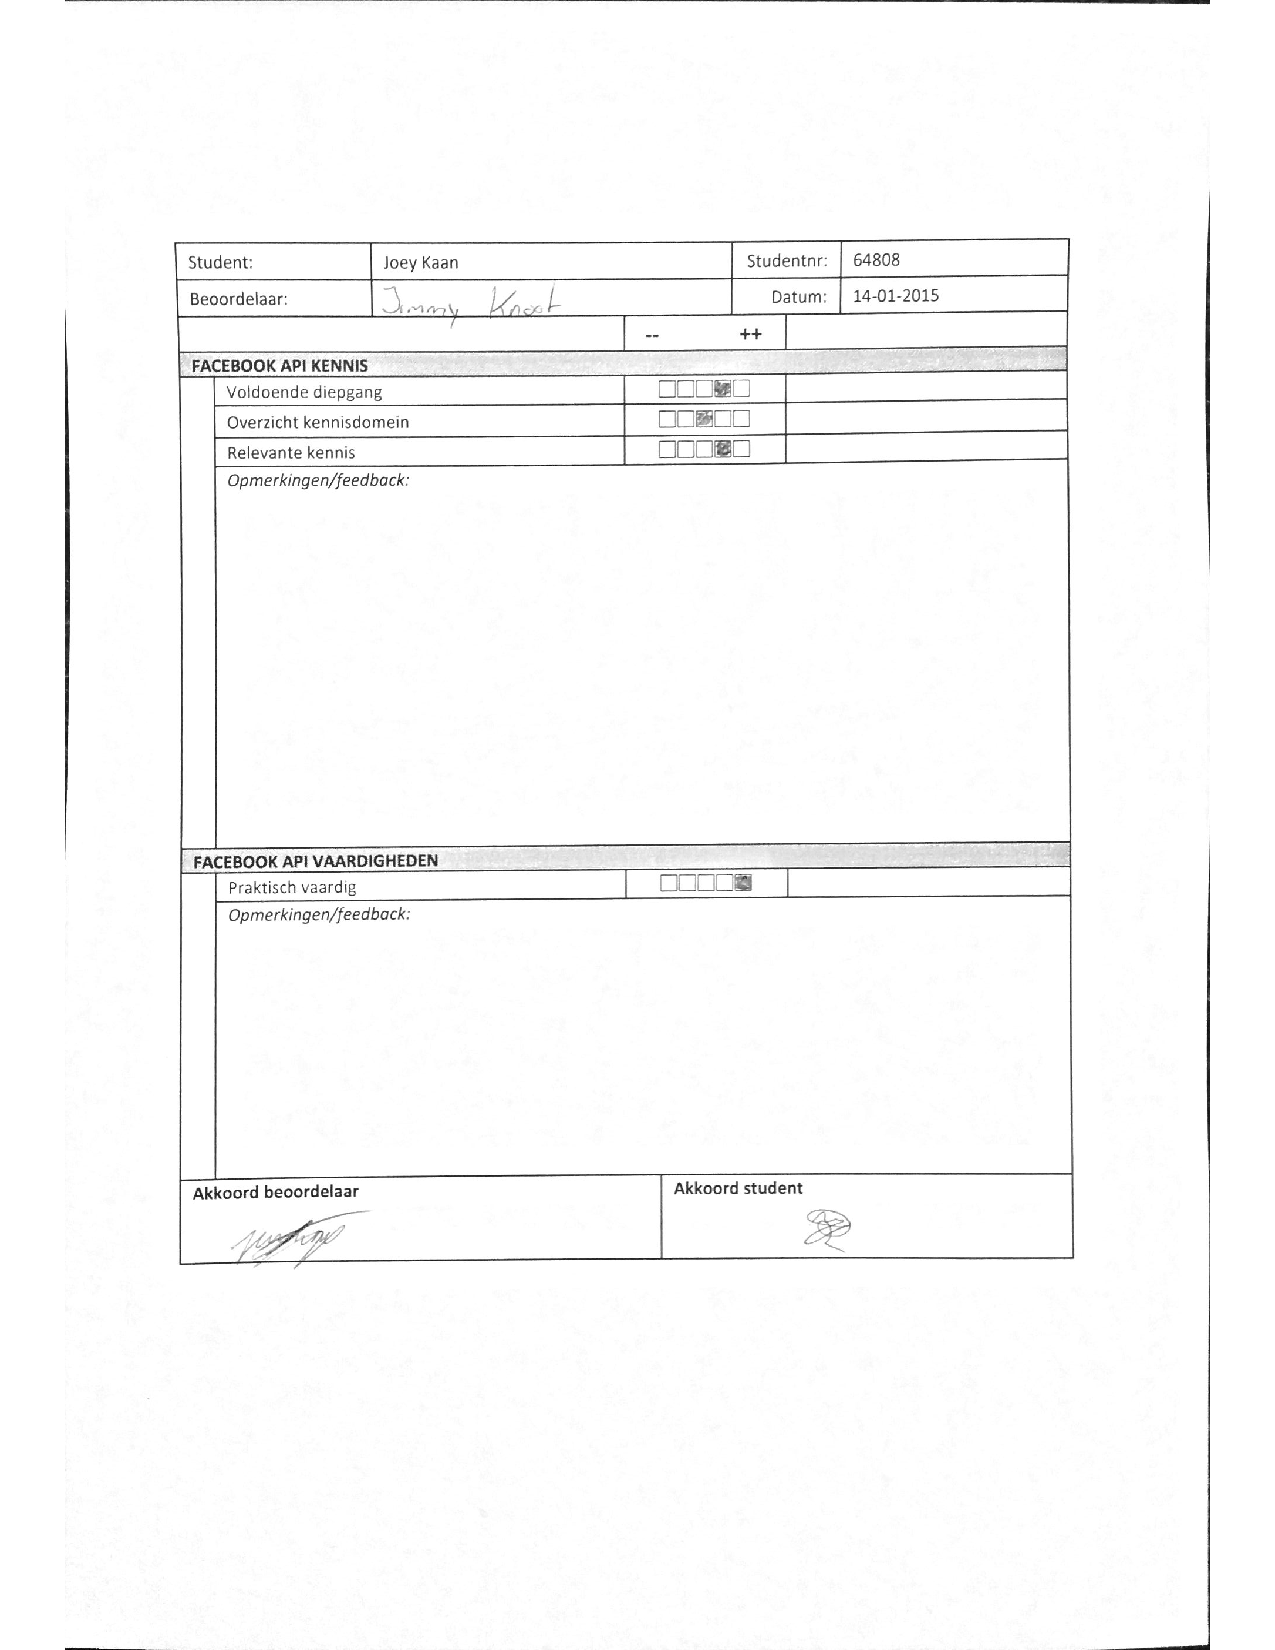
\includepdf[pages={1}, scale=0.65, pagecommand=\thispagestyle{fancy}]{attachments/beoordelingsformulier-fapi.pdf}

\paragraph{Bewijs 2: Uitwerking}
Hieronder staat de code die momenteel wordt gebruikt om te communiceren met de Facebook API. De motivatie om de uitwerking op te nemen als bewijs is omdat het invullen van een formulier natuurlijk niets zegt als de uitwerking niet ook aanwezig is.

\begin{lstlisting}[caption=Facebook API interactie]
/**
 * This class is responsible for interacting with the different social media API's to retrieve data about an user.
 */
SocialMediaDataRetriever = {
    processFacebookProfiles: function () {
        var profilesToSend = this.getNotProcessedProfiles('facebook', 50);

        var facebookIds = _.map(profilesToSend, function (facebookProfile) {
            return facebookProfile.data.facebookId;
        });

        var graphFacebookUrl = 'https://graph.facebook.com/?metadata=1&ids=' + facebookIds.join(",");

        HTTP.call('GET', graphFacebookUrl, function (err, response) {
            if(err) throw err;

            var result = JSON.parse(response.content);
            _.each(profilesToSend, function(facebookProfile) {
                var currentResultSet = result[facebookProfile.data.facebookId];

                var updateQuery = {};
                updateQuery.$set = {};
                updateQuery.$set['facebookLastUpdatedAt'] = new Date();

                updateQuery.$set['data.facebookId'] = currentResultSet['id'];

                if (currentResultSet['first_name']) {
                    updateQuery.$set['data.firstName'] = currentResultSet['first_name'];
                }

                if (currentResultSet['last_name']) {
                    updateQuery.$set['data.lastName'] = currentResultSet['last_name'];
                }

                if (currentResultSet['locale']) {
                    updateQuery.$set['data.locale'] = currentResultSet['locale'];
                }

                if (currentResultSet['gender']) {
                    updateQuery.$set['data.sex'] = currentResultSet['gender'];
                }

                if (currentResultSet['name']) {
                    updateQuery.$set['data.fullName'] = currentResultSet['name'];
                }

                Profiles.updateProfile(facebookProfile._id, updateQuery);
            });
        });
    }
};
\end{lstlisting}

Het deel waar daadwerkelijk met de Facebook API contact wordt gelegd begint op lijn 14. Naar het eindpunt wordt een lijst met ID's verstuurd. Er wordt eerst gekeken of er een error is, zo niet dan worden de resultaten uitgelezen en in de database verwerkt. De uitwerking lijkt weliswaar weinig, maar er is veel onderzoeken en refactoren aan vooraf gegaan.

\clearpage

\subsection{Meteor, een JavaScript framework}
Het leerdoel dat hierbij hoort: Meteor leren kennen door middel van een applicatie te maken die real-time informatie weergeeft over een klant’s social media kanalen aan meerdere eind-gebruikers, dit wordt verwezenlijkt door Meteor’s collections en het publish-subscribe pattern te gebruiken.

\subsubsection{STARRT Formulier}
\begin{tabularx}{\textwidth}{| l | X |}
\hline
\multicolumn{2}{|l|}{Academie: Academie voor Technologie \& Innovatie } \\
\hline
\multicolumn{2}{|l|}{Opleiding: HBO-ICT } \\
\hline
\multicolumn{2}{|l|}{Studentnaam: Joey Kaan \hspace{35pt} Studentnummer: 64808} \\
\hline
\multicolumn{2}{|l|}{Stagedocent: D. de Waard} \\
\hline
\multicolumn{2}{|p{\textwidth-1in}|}{Leerdoel/competentie: Meteor leren kennen door middel van een applicatie te maken die real-time informatie weergeeft over een klant’s social media kanalen aan meerdere eind-gebruikers, dit wordt verwezenlijkt door Meteor’s collections en het publish-subscribe pattern te gebruiken.} \\
\hline
\multicolumn{2}{|l|}{Cursus: Meewerkstage \hspace{35pt} Cursuscode: CU06322} \\
\hline
\multicolumn{2}{|l|}{Datum: \today} \\
\hline
\multicolumn{2}{|l|}{
\begin{minipage}{0.9\columnwidth}
Titel en nummer van bewijs/bewijzen:
\begin{itemize}
\item Bewijs 1: Uitleg publish-subscribe pattern \& Meteor's collections
\item Bewijs 2: Beoordelingsformulier
\end{itemize}
\end{minipage}
} \\ [50pt]
\hline
\multicolumn{2}{|l|}{Oordeel: } \\
\hline
S & Geef voorbeelden van opdrachten (situaties) waarmee je kunt aantonen dat je de competentie hebt verworven. Beschrijf kort wat er aan de hand was of om welke opdracht het ging.
\newline
\newline
Tijdens het programmeren heb ik meerdere keren iets veranderd waardoor het beter samenwerkte met Meteor, dit was dan gemaakt door een van mijn mede-programmeurs. Bijvoorbeeld als het gaat om events; als je bijvoorbeeld klikt op een knop moet deze een bepaalde actie uitvoeren. Meteor verzorgt hier zelf functionaliteit voor die het makkelijker maakt om events af te handelen. Eerst werden events nog op de `oude` jQuery manier gedaan, naast het feit dat deze langzamer zijn dan de Meteor manier is het ook nog eens veel duidelijker als het gedaan wordt zoals de specificatie van Meteor beschrijft.
\\
\hline
T & Beschrijf de exacte rol/taak die jij had. Geef aan of het om een complexe taak ging en waaruit dat bleek. Wat moest jij doen?
\newline
\newline
Mijn rol was programmeur bij Profile2Connect, dit komt er op neer dat ik functionaliteit toe voeg aan Profile2Connect. Deze functionaliteit werd vastgesteld door de opdrachtgever, de programmeurs hadden hier zelf input in. Tijdens deze meetings is het vaak lastig om in te schatten hoeveel tijd iets kost en wat de meerwaarde zal zijn voor de klant. Naast developer moest ik dus ook keuzes maken over welke functionaliteit wel in Profile2Connect komt en welke niet, hierbij moet er dus gekeken worden vanuit het oog van de klant en dat is vaak lastig als je zelf dag in dag uit bezig bent met programmeren. Dit zorgde er dus voor dat sommige dingen wat langer duurden, want er moest goed overlegd worden en vaak ook nog met buitenstaanders die dan de rol van klant op zich namen.
\\
\hline
A & Beschrijf de activiteiten die jij achtereenvolgens hebt ondernomen in het kader van deze opdracht. Wat heb je concreet gedaan?
\newline
\newline
Tijdens het oplossen van het probleem met de Facebook API heb ik een aantal activiteiten uitgevoerd:

\begin{itemize}
\item Inlezen over Meteor; Discover Meteor boek doorlopen.
\item Keuzes maken over functionaliteit die beschikbaar zal zijn in Profile2Connect
\item Functionaliteit programmeren
\end{itemize}

\\
\hline
R & Beschrijf het resultaat van de opdracht en hoe de betrokkenen er op reageerden. Wat is er vervolgens met dat resultaat gebeurd?
\newline
\newline
Het programmeren met Meteor ging heel erg snel en fijn. Het was een nieuw platform en toen we ermee begonnen was het zelfs nog in beta. Daar in tegen hebben we overigens weinig tegenslag gehad, alleen omdat er nog weinig over bekend is liggen sommige memory leaks niet echt voor de hand. We hebben gebruik gemaakt van een monitoring tool genaamd Kadira, hiermee konden we gemakkelijk zien of er enige memory leaks aanwezig waren of niet. De opdrachtgever was heel blij met het feit dat er zo snel nieuwe functionaliteit toegevoegd werd en de klanten die Profile2Connect gebruikten waren ook erg blij met het resultaat.
\\
\hline
R & Wat heb je ervan geleerd? Wat zou je volgende keer anders aanpakken en waarom?
\newline
\newline
Ik heb een aantal dingen geleerd tijdens het werken aan deze competentie:
\begin{itemize}
\item Als software in beta is, betekent niet dat het niet in productie te gebruiken is.
\item Het is zeker de tijd en moeite waard om nieuwe technologiën te ontdekken.
\item Het is altijd belangrijk om uit het oogpunt van de klant te denken, deze moet het immers gebruiken.
\item Overleggen met de mede-programmeurs over het voltooide programmeerwerk zodat er geen dubbel werk verricht wordt.
\end{itemize}

Zelf ben ik zeer tevreden over mijn kennis van Meteor. Natuurlijk kende ik al JavaScript, maar het is heel wat anders om hier 8 uur per dag mee bezig te zijn dan soms een simpele animatie o.i.d. te maken. Ik ben dus trots dat ik JavaScript en Meteor zo goed heb leren gebruiken in maar 5~ maanden tijd.
\\
\hline
T & Geef een voorbeeld van een andere situatie waarin je deze competentie kunt toepassen
\newline
\newline
JavaScript frameworks worden steeds populairder, veel bedrijven gebruiken deze frameworks en er komen steeds meer bedrijven bij. Als bedrijf is het belangrijk om snel software op te kunnen leveren en Meteor helpt hier zeker bij. In de toekomst zullen meer bedrijven op zoek gaan naar Meteor developers en daarom komt het zeer handig uit
\\
\hline
\end{tabularx}

\subsubsection{Bewijzen}
\paragraph{Bewijs 1: Uitleg publish-subscribe pattern \& Meteor's collections}
\begin{center}
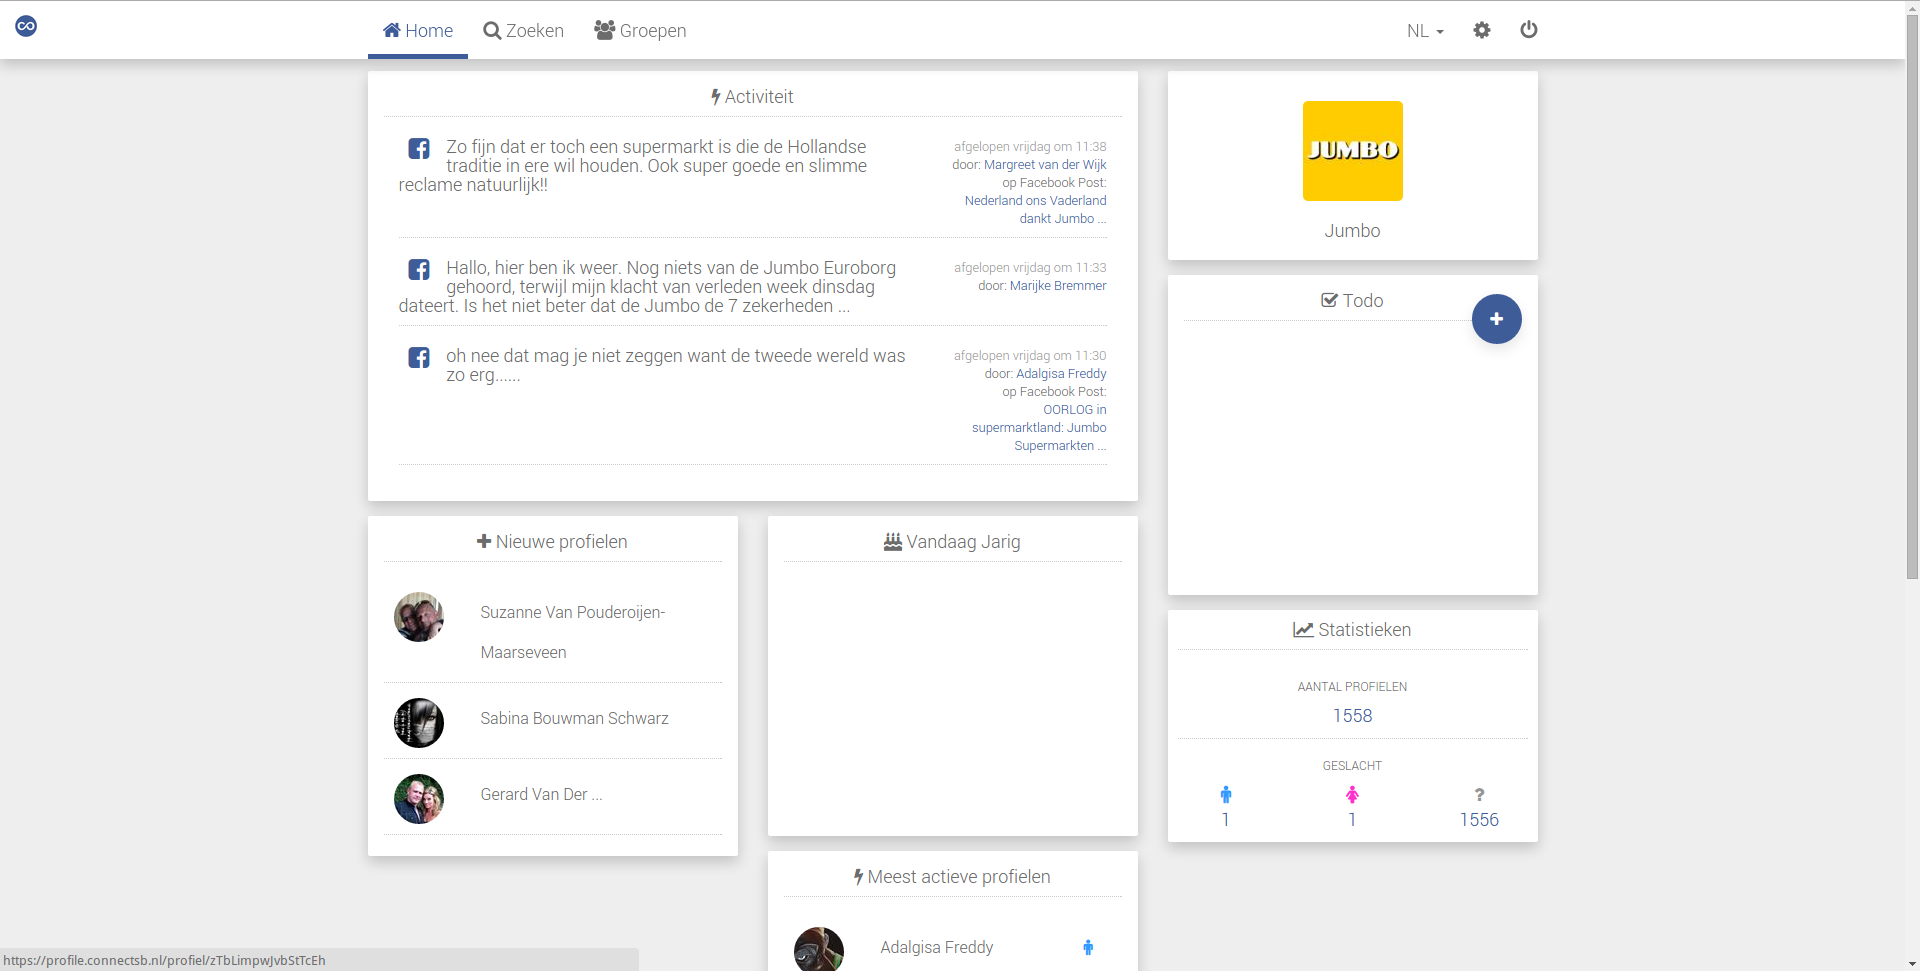
\includegraphics[width=\textwidth,keepaspectratio]{attachments/profile2connect}
\caption{\label{fig:profile2connect-home} Profile2Connect welkomst pagina}
\end{center}

De gegevens die te zien zijn op deze pagina komen van verschillende publicaties. Zo zie je bijvoorbeeld een logo van de op dit moment ingelogde klant(rechts boven in), de updates (links boven in) en dan nog een aantal overige categoriën zoals nieuwe profielen en meest actieve profielen. Al deze categoriën zijn allemaal aparte publicaties, dit wordt gedaan omdat je dan nooit meer data beschikbaar hebt op de client dan dat je nodig hebt. Het optellen van de totalen wordt ook op de server gedaan, je wilt natuurlijk niet alle profielen van een klant op de welkomst pagina beschikbaar maken. Hierdoor zou de applicatie heel lang kunnen doen over het laden, omdat hij al deze profielen uit de database zou moeten halen.

Hoe het publish-subscribe pattern precies werkt kan beter uitgelegd worden aan de hand van een paar code snippets:
\begin{lstlisting}[caption=Profielen publiceren]
// Publish all profiles
Meteor.publish("profiles", function () {
    return Profiles.find(filter, specifiers);
});
\end{lstlisting}

\begin{lstlisting}[caption=Profielen abonneren]
// Subscribe to profiles publication
Meteor.subscribe('profiles');
\end{lstlisting}

De code hierboven is aangepast zodat deze gemakkelijker te lezen zou zijn. Alle data die je beschikbaar wil maken in Meteor aan de front-end, begint met een publicatie, een publicatie gebeurd altijd aan de server kant. Je publiceert dus een bepaalde \gls{collection} door middel van de publish functie. Als je hier niet op abbonneert dan gaat de data `verloren`. Als je dus abbonneert op de publicatie kun je later in de code de inhoud van de gepubliceerde \gls{collection} ophalen. Dit gebeurd op deze manier:

\begin{lstlisting}[caption=Profielen ophalen]
// Retrieve profiles
var profiles = Profiles.find().fetch();
\end{lstlisting}

De profiles array zal dan gevuld zijn met de data die je hebt gepubliceerd op de server. Als je niet abbonneert op de publicatie zal de profiles array leeg zijn. Op deze manier maakt Meteor het heel erg gemakkelijk om aan te geven waar welke data aanwezig is. Je ziet hier dat er uit wordt gegaan van een Profiles \gls{collection}. Deze collectie moet natuurlijk ook ergens gedefinieerd worden. Dit wordt op deze manier gedaan:

\begin{lstlisting}[caption=Profielen collectie aanmaken]
// Create profiles collection
Profiles = new Meteor.Collection('profiles');
\end{lstlisting}

Zoals je ziet wordt deze collectie opgeslagen in een variabele genaamd Profiles. Zo is het dus mogelijk om ergens anders in de code methodes uit te voeren op deze variabele zoals je kunt zien in de bovenstaande code-snippets.

De reden dat dit is opgenomen in de bewijzen is door het uitleggen van de principes zoals publish en subscribe en Meteor's collection dat hiermee de expertise wat betreft Meteor wordt aangetoond.
\paragraph{Bewijs 2: Beoordelingsformulier}
Tijdens het programmeren met Meteor heeft Jimmy Knoot mijn programmeerwerk beoordeeld. Bij ConnectSB is het de gewoonte om \gls{peerreviews} te houden. Hij heeft zelf ook veel ervaring met Meteor dus daarom is hij de persoon om mij op mijn Meteor kennis te beoordelen.
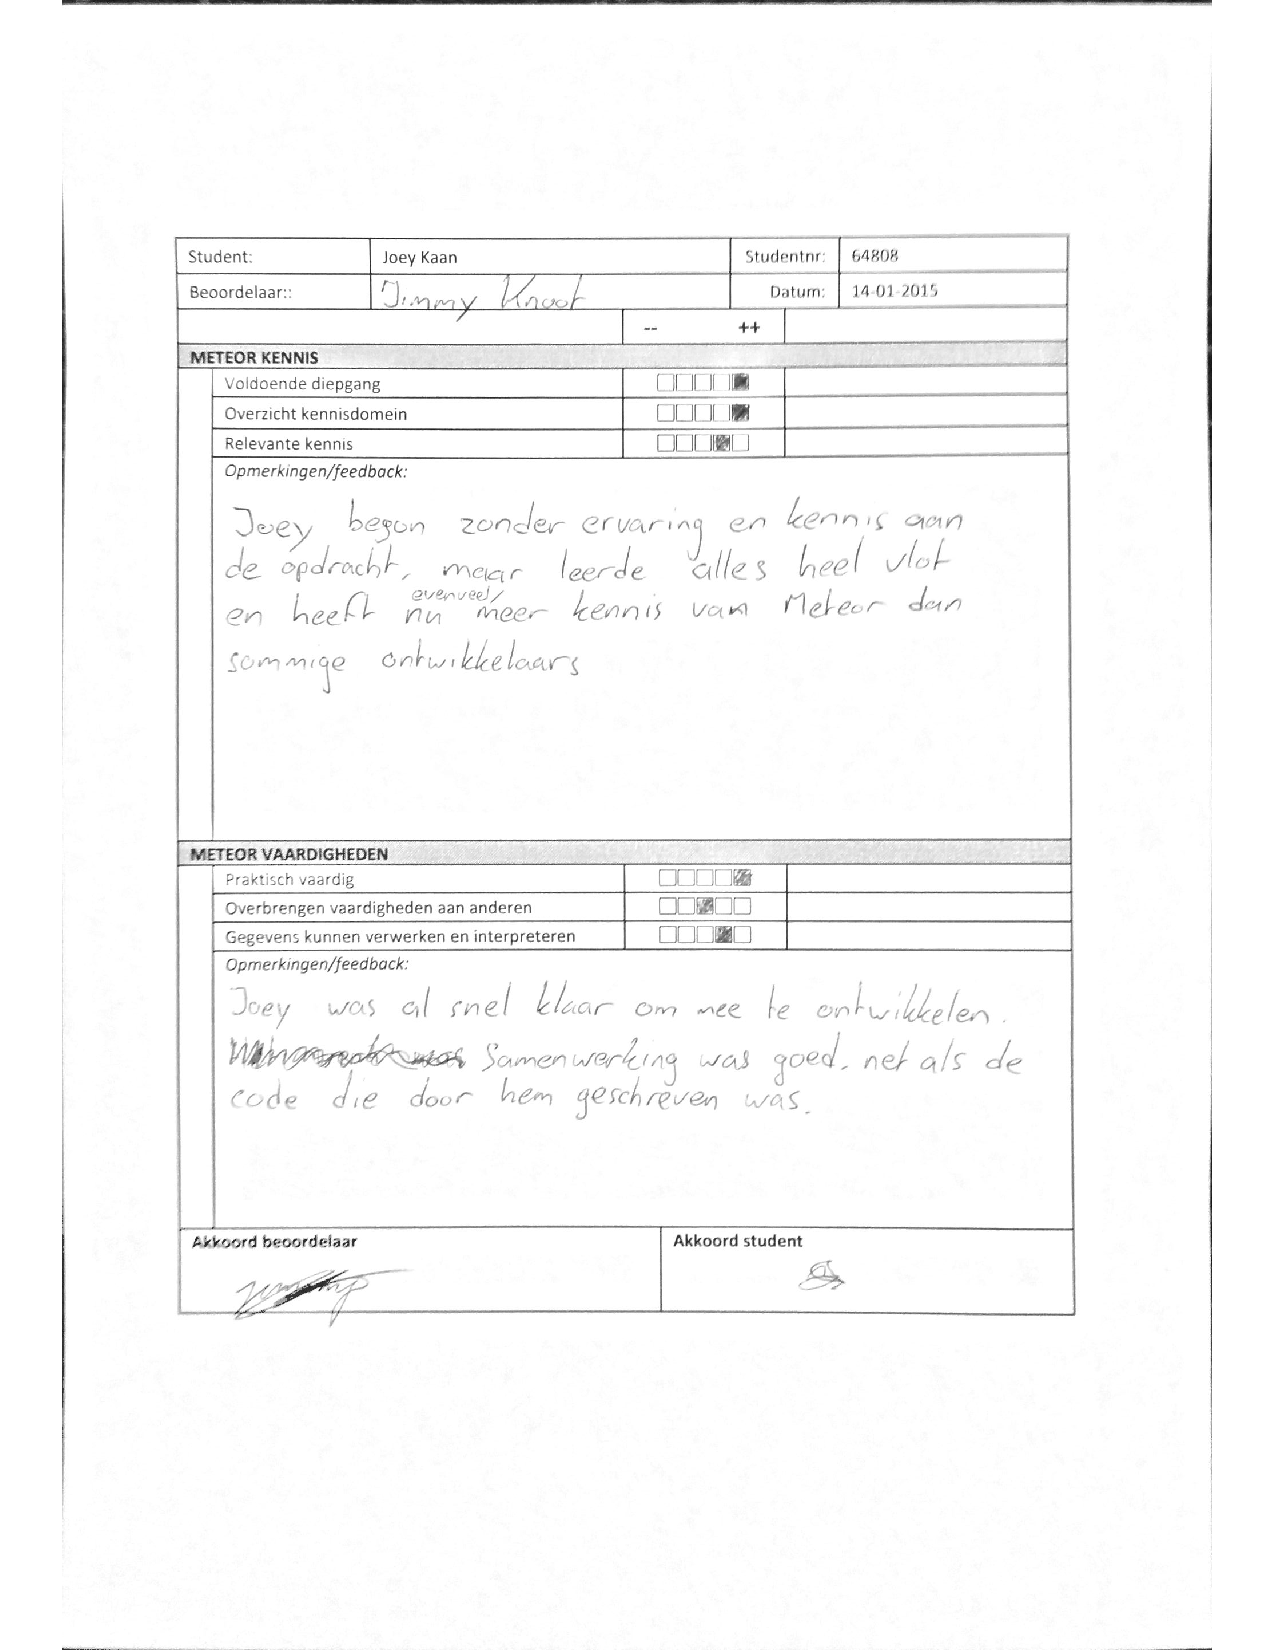
\includepdf[pages={1}, scale=0.65, pagecommand=\thispagestyle{fancy}]{attachments/beoordelingsformulier-meteor.pdf}

\clearpage

\subsection{Versiebeheer}
Het desbetreffende leerdoel is: Versiebeheer volgens de \gls{gitflow} workflow gebruiken zodat er altijd een fout vrije en uitrolbare versie van de applicatie beschikbaar is en als er een fout optreedt deze snel weer ongedaan gemaakt kan worden door naar een vorige versie terug te keren.

\subsubsection{STARRT Formulier}
\begin{tabularx}{\textwidth}{| l | X |}
\hline
\multicolumn{2}{|l|}{Academie: Academie voor Technologie \& Innovatie } \\
\hline
\multicolumn{2}{|l|}{Opleiding: HBO-ICT } \\
\hline
\multicolumn{2}{|l|}{Studentnaam: Joey Kaan \hspace{35pt} Studentnummer: 64808} \\
\hline
\multicolumn{2}{|l|}{Stagedocent: D. de Waard} \\
\hline
\multicolumn{2}{|p{\textwidth-1in}|}{Leerdoel/competentie: Versiebeheer volgens de \gls{gitflow} gebruiken zodat er
altijd een fout vrije en uitrolbare versie van de applicatie beschikbaar is en als
er een fout optreedt deze snel weer ongedaan gemaakt kan worden door naar
een vorige versie terug te keren.} \\
\hline
\multicolumn{2}{|l|}{Cursus: Meewerkstage \hspace{35pt} Cursuscode: CU06322} \\
\hline
\multicolumn{2}{|l|}{Datum: \today} \\
\hline
\multicolumn{2}{|l|}{
\begin{minipage}{0.9\columnwidth}
Titel en nummer van bewijs/bewijzen:
\begin{itemize}
\item Bewijs 1: Content2Connect commit geschiedenis
\item Bewijs 2: Gitflow CLI
\end{itemize}
\end{minipage}
} \\ [50pt]
\hline
\multicolumn{2}{|l|}{Oordeel: } \\
\hline
S & Geef voorbeelden van opdrachten (situaties) waarmee je kunt aantonen dat je de competentie hebt verworven. Beschrijf kort wat er aan de hand was of om welke opdracht het ging.
\newline
\newline
De opdracht was Content2Connect. Deze was zo ver dat er een versie 1.0 kon worden uitgebracht. \\
\hline
T & Beschrijf de exacte rol/taak die jij had. Geef aan of het om een complexe taak ging en waaruit dat bleek. Wat moest jij doen?
\newline
\newline
Mijn rol was het klaarmaken van Content2Connect voor de release, Content2Connect te releasen en daarna deze ook te beheren. Met beheren wordt bedoeld of de release goed is gelukt, of alle functies ook werken op de productie server. Zo niet dan zal hier wat aanpassingen aan gedaan moeten worden. Hiernaast moet ook de feedback van klanten en van de interne gebruikers van ConnectSB worden verwerkt en bugs gefixed worden naarmate deze worden gevonden.
\\
\hline
A & Beschrijf de activiteiten die jij achtereenvolgens hebt ondernomen in het kader van deze opdracht. Wat heb je concreet gedaan?
\begin{itemize}
\item Functionaliteit voor Content2Connect afmaken.
\item Online zetten voor testen op test omgeving.
\item Test periode doorlopen waarbij getest wordt door management en community management.
\item Feedback verwerken van de test periode.
\item Online zetten op de productie omgeving.
\item Bugs gefixed die gaande weg ontdekt werden.
\item Nieuwe branch aangemaakt met de volgende naam: hotfix-testbugs.
\item Bugs opgelost in deze branch.
\item Hotfix-testbugs branch gemerged met master branch
\end{itemize}
\\
\hline
R & Beschrijf het resultaat van de opdracht en hoe de betrokkenen er op reageerden. Wat is er vervolgens met dat resultaat gebeurd?
\newline
\newline
Het resultaat was een volledig werkende versie van  Content2Connect, de eerste dag hadden er al twee klanten gebruik gemaakt van het platform en dit was allemaal succesvol verlopen. De klanten waren heel enthousiast over het platform, het werkte heel prettig en het was vooral heel overzichtelijk.
\\
\hline
R & Wat heb je ervan geleerd? Wat zou je volgende keer anders aanpakken en waarom?
\newline
\newline
Tijdens het klaarmaken van Content2Connect voor de release heb ik geleerd dat het continue testen heel erg belangrijk is. Bij ConnectSB is er nog maar sinds kort de regel dat er tests geschreven moeten worden en Content2Connect had deze tests nog niet. In Content2Connect worden er verschillende notificaties verstuurd met hierbij bijbehorende emails. De emails werden soms wel verzonden en soms niet bleek na de test periode. Als hiervoor tests geschreven waren had ik heel erg gemakkelijk kunnen zien waar de fout zat. Zo heb ik toen nog wel tests geschreven voor de email functie en hiermee kon ik dus heel gemakkelijk ook zien waar de fout zat.

\newline
Ik was zelf zeer tevreden met het resultaat, dit was de eerste keer dat ik bij zo'n groot project van begin tot eind aanwezig ben geweest, ook heb ik het gehele project helemaal zelf geprogrammeerd. Ik zou overigens wel willen dat ik wat langer over bepaalde zaken had nagedacht voordat ik een oplossing ging programmeren, omdat nu een paar dingen wat onduidelijk zullen zijn voor de volgende persoon die er aan zal gaan werken. Ik had daarna geen tijd meer om deze dingen aan te passen, omdat ik toen al verder moest met wat anders.
\\
\hline
T & Geef een voorbeeld van een andere situatie waarin je deze competentie kunt toepassen
\newline
\newline
Deze competentie is eigenlijk te gebruiken gedurende de hele levensduur van de software. De \gls{gitflow} workflow gaat niet alleen over software die al in gebruik genomen wordt. Het is een workflow die het makkelijk maakt om aan aparte features te werken zonder dat de toestand van het development werk en de toestand van de code die productie gereed is wordt aangetast.
\\
\hline
\end{tabularx}
Voor Content2Connect moesten een aantal belangrijke fixes gebeuren, deze hadden hoge prioriteit. Deze komen volgens de \gls{gitflow} workflow dan op zogenaamde feature branches. Er is geen speciale conventie voor hoe deze feature branches moeten heetten maar heel veel bedrijven houden de volgende conventie aan: feature/[feature-naam], dit heb ik dus ook gedaan. Mijn branch voor deze belangrijke fixes heet daarom ook feature/important-fixes. Bij ConnectSB wordt gewerkt met \gls{redmine} en hierbij kan er prioriteit gegeven worden aan bepaalde issues. Deze hoge prioriteit komt dus ook van \gls{redmine}.

Voor een grote hoeveelheid met kleine issues is het in mijn belevenis beter om een branch te maken die deze allemaal bevat. Veel bedrijven houden zich ook aan het aanmaken van één branch voor elke issue, maar dit is naar mijn idee geen goed idee. Als een issue natuurlijk best wel uitgebreid is en je waarschijnlijk kleine taken zult hebben is dit een goed idee, maar als je één issue moet doen die hooguit 5 minuten duurt is dit het natuurlijk niet echt waard.

Ik moest in Content2Connect bij het overzicht van één bestelling de titel toevoegen van de bestelling. Hiervoor wordt er dan een branch gemaakt genaamd feature/change-\#2318 want de issue heet op \gls{redmine} Change \#2318. Change is dan de categorie en \#2318 is het nummer van de issue.

Dit is dus nu gedaan voor elke issue die op \gls{redmine} stond. Deze branches komen eigenlijk nooit op de centrale repository. Deze kunnen gepusht worden als dat nodig is, bijvoorbeeld als iemand mee moet helpen om aan een bepaalde feature mee te werken. Features zullen meest van de tijd, in ieder geval in mijn situatie, werk bevatten voor één persoon dus de feature branches hoeven dan nooit gepusht te worden.

Vandaag is er een release voor Content2Connect uitgebracht. Dit is versie v0.9, hier wordt dan een tag voor aangemaakt op de master en dan kan deze in productie gezet worden.

\gls{gitflow} werkt vooral heel goed als je bijvoorbeeld bezig bent aan nieuwe functionaliteit, maar je baas zegt dat er even snel wat anders moet gebeuren. Je maakt een nieuwe feature branch aan, commit daar alles op. Deze merge je dan met de develop branch en indien nodig kan deze naar master voor een nieuwe release. Alle changes waar je dan eerst mee bezig was kun je dan heel gemakkelijk weer.

\subsubsection{Bewijzen}
\paragraph{Bewijs 1: Content2Connect commit geschiedenis}
Hieronder is een deel van de commit geschiedenis te zien van Content2Connect, aan de hand van deze afbeelding zal ik uitleggen waarom de \gls{gitflow} goed werkt en hoe je kan zien dat dit de \gls{gitflow} is. Hiermee kan dus aangetoond worden dat er daadwerkelijk met de \gls{gitflow} is gewerkt.

\vspace{3mm}

\begin{minipage}{0.5\textwidth}
\begin{figure}[H]
\begin{adjustwidth}{-0.6cm}{}
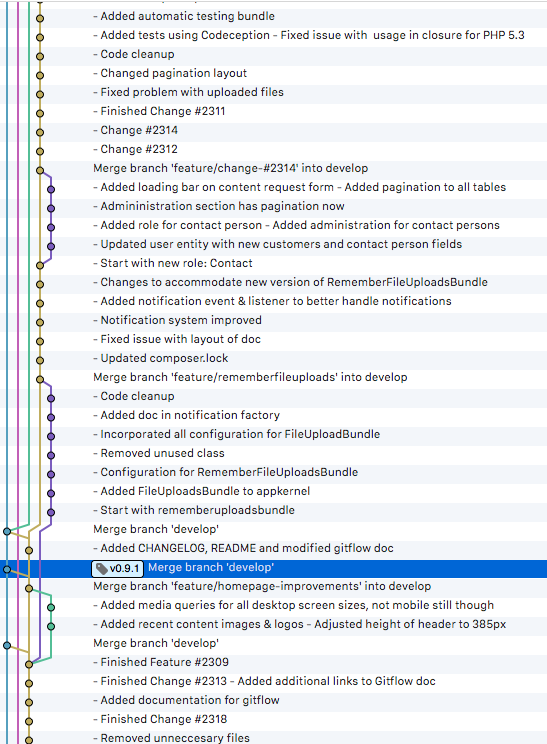
\includegraphics[width=8cm,height=8cm,keepaspectratio]{attachments/Content2Connect-history}
\caption{\label{fig:commit-history} Content2Connect commit geschiedenis}
\end{adjustwidth}
\end{figure}
\end{minipage} \hfill
\begin{minipage}{0.45\textwidth}
\begin{footnotesize}
Een overzicht van wat de verschillende kleuren lijnen betekenen volgt hieronder:
\begin{itemize}
\item Blauw: master branch
\item Geel: develop branch
\item Roze: prod branch
\item Overige kleuren: feature branches
\end{itemize}
Voorbeelden van zogenaamde feature-branches zijn te zien bij de groene en paarse lijnen. Als de feature klaar is worden deze gemerged met develop, kenmerkend aan het bericht: merge branch feature/[naam] into develop. Ook is te zien dat er aan verschillende features tegelijkertijd gewerkt kan worden. (paars en groen). Dat is een groot voordeel van de Gitflow workflow.

In de afbeelding is ook nog een voorbeeld te zien van een release. Er wordt een tag aangemaakt, in dit geval v0.9.1 op de master branch. Daarvoor wordt eerst de develop branch goed getest zodat er geen fouten in zitten. Op deze manier bevat de master branch altijd de code die release klaar is. Dit maakt het gemakkelijk voor de developers om te ontwikkelen zonder zich druk te hoeven maken dat er iets op productie verkeerd kan gaan.
\end{footnotesize}
\end{minipage}

\paragraph{Bewijs 2: Gitflow CLI}
Tijdens het werken met Gitflow had ik door dat ik soms vergat om voor een nieuwe feature een feature-branch te maken, of om een nieuwe tag te maken als er een nieuwe release plaats ging vinden. Ik ben toen op zoek gegaan naar een programma dat dit gemakkelijker zou maken. Toen heb ik dus de Gitflow CLI\cite{gitflowcli} gevonden. Deze maakt het super gemakkelijk om volgens de \gls{gitflow} te werken. Niet alleen wordt het super makkelijk, maar het garandeert ook dat het aan de standaarden van de \gls{gitflow} voldoet, dit is ook de reden dat dit is opgenomen bij de bewijzen.

Een voorbeeld van hoe ik mijn project heb opgezet met dit programmaatje volgt hieronder:

\begin{lstlisting}[caption=Aanmaken Gitflow project]
// Initialize git
git init
// Initiliaze Gitflow CLI
git flow init -d
// Start a new feature, creates branch called feature/important-fixes
git flow feature start important-fixes
\end{lstlisting}

\clearpage

\subsection{Functioneel ontwerp}
Ik heb voor Content2Connect natuurlijk een functioneel ontwerp, vanaf nu FO, op moeten zetten, dit FO is overigens niet zo gestructureerd zoals wordt verwacht op de HBO-ICT opleiding. Voor de opdrachtgever was het belangrijk dat alle functionele eisen in het FO zijn opgenomen en dat alles van de uitwerking duidelijk was. Bij ConnectSB werken ze nooit een volledig FO uit, omdat dit wordt gezien als zonde van de tijd. De standaard layout van een FO is dus als volgt:
\begin{itemize}
\item Algemene Informatie
\item Eisen onderverdeeld in Front-end en Back-end
\item Flow
\item Oplevering
\item Eventuele extra's
\end{itemize}
Het is allemaal vrij logisch wat er bedoelt wordt met die punten, overigens is er een punt die misschien enige vraagtekens oproept. Het gaat dan om de `Flow`. Dit wil zeggen wat een gebruiker ervaart als ze gebruik maken van het product. Zo was het dus bijvoorbeeld bij Content2Connect het proces van credits kopen, content kopen, deze goedkeuren/afkeuren en deze als laatste stap downloaden. Hoe werkt dit precies en wat komt hier allemaal bij kijken zijn een aantal vragen die je hierbij moet stellen.

\subsubsection{STARRT Formulier}
\begin{tabularx}{\textwidth}{| l | X |}
\hline
\multicolumn{2}{|l|}{Academie: Academie voor Technologie \& Innovatie } \\
\hline
\multicolumn{2}{|l|}{Opleiding: HBO-ICT } \\
\hline
\multicolumn{2}{|l|}{Studentnaam: Joey Kaan \hspace{35pt} Studentnummer: 64808} \\
\hline
\multicolumn{2}{|l|}{Stagedocent: D. de Waard} \\
\hline
\multicolumn{2}{|p{\textwidth-1in}|}{Leerdoel/competentie: Functioneel ontwerp opstellen zodat deze makkelijk leesbaar en begrijpbaar is voor een persoon die niets af weet van de te maken software en dat de opdrachtgever gemakkelijk zijn eisen in het functioneel ontwerp terug kan vinden.} \\
\hline
\multicolumn{2}{|l|}{Cursus: Meewerkstage \hspace{35pt} Cursuscode: CU06322} \\
\hline
\multicolumn{2}{|l|}{Datum: \today} \\
\hline
\multicolumn{2}{|l|}{
\begin{minipage}{0.9\columnwidth}
Titel en nummer van bewijs/bewijzen:
\begin{itemize}
\item Bewijs 1: Uitwerking
\end{itemize}
\end{minipage}
} \\ [50pt]
\hline
\multicolumn{2}{|l|}{Oordeel: } \\
\hline
S & Geef voorbeelden van opdrachten (situaties) waarmee je kunt aantonen dat je de competentie hebt verworven. Beschrijf kort wat er aan de hand was of om welke opdracht het ging.
\newline
\newline
De opdracht was een functioneel ontwerp maken. \\
\hline
T & Beschrijf de exacte rol/taak die jij had. Geef aan of het om een complexe taak ging en waaruit dat bleek. Wat moest jij doen?
\newline
\newline
Mijn rol was een functioneel ontwerp opstellen voor Content2Connect.
\\
\hline
A & Beschrijf de activiteiten die jij achtereenvolgens hebt ondernomen in het kader van deze opdracht. Wat heb je concreet gedaan?
\begin{itemize}
\item Gesprek hebben met opdrachtgever over de eisen van Content2Connect (Paul)
\item Concept versie maken functioneel ontwerp aan de hand van eisen ConnectSB en opdrachtgever (Paul)
\item Bespreken concept versie opdrachtgever (Paul)
\item Opmerkingen opdrachtgever verwerken in functioneel ontwerp
\item Bespreken volgende versie functioneel ontwerp
\item Opmerkingen opdrachtgever verwerken in functioneel ontwerp en afronden
\end{itemize}
\\
\hline
R & Beschrijf het resultaat van de opdracht en hoe de betrokkenen er op reageerden. Wat is er vervolgens met dat resultaat gebeurd?
\newline
\newline
Het resultaat was een functioneel ontwerp dat voldoet aan de eisen van ConnectSB. Dit resultaat is toen door de opdrachtgever (Paul) bekeken en goed bevonden.
\\
\hline
R & Wat heb je ervan geleerd? Wat zou je volgende keer anders aanpakken en waarom?
\newline
\newline
Op de HZ wordt een functioneel ontwerp met veel overbodige diagrammen gemaakt. Dit kost veel tijd voor de developer en ook voor de opdrachtgever zelf. Tegenwoordig ligt de focus op het leveren van software en alle tijd die daarvoor gebruikt kan worden en niet voor iets anders is welkom. Ik vind het ook een stuk prettiger werken, want met deze vorm van een functioneel ontwerp is alles duidelijk zonder enige zaken waar niemand naar kijkt.

\newline
Ik ben zelf heel erg tevreden met het resultaat, in relatief korte tijd een goed en duidelijk functioneel ontwerp opgeleverd. Tijdens het programmeren kwam deze ook goed van pas, want er was nooit echt onduidelijkheid.
\\
\hline
T & Geef een voorbeeld van een andere situatie waarin je deze competentie kunt toepassen
\newline
\newline
Een functioneel ontwerp schrijven is een heel belangrijk onderdeel van het ontwikkelen van software en zal op de een of andere manier altijd wel aan bod komen. Deze competentie kan dus altijd gebruikt worden als developer en alle ervaring hiermee is welkom.
\\
\hline
\end{tabularx}

\subsubsection{Bewijzen}

\paragraph{Bewijs 1: Uitwerking}
De uitwerking wordt natuurlijk opgenomen in de bewijzen, hiermee kan samen met de beoordeling worden aangetoond dat deze competentie behaald is. De uitwerking is aanwezig in de bijlage, Bijlage D - Content2Connect FO

\paragraph{Bewijs 2: Beoordelingsformulier}
Content2Connect was een idee van Paul Brinkhof, hij zit in het management bij ConnectSB. Destijds heb ik toen ook het functioneel ontwerp gemaakt en hij was dus de opdrachtgever bij het project. Daarom heeft hij een beoordeling gemaakt van de kwaliteit van het functionele ontwerp

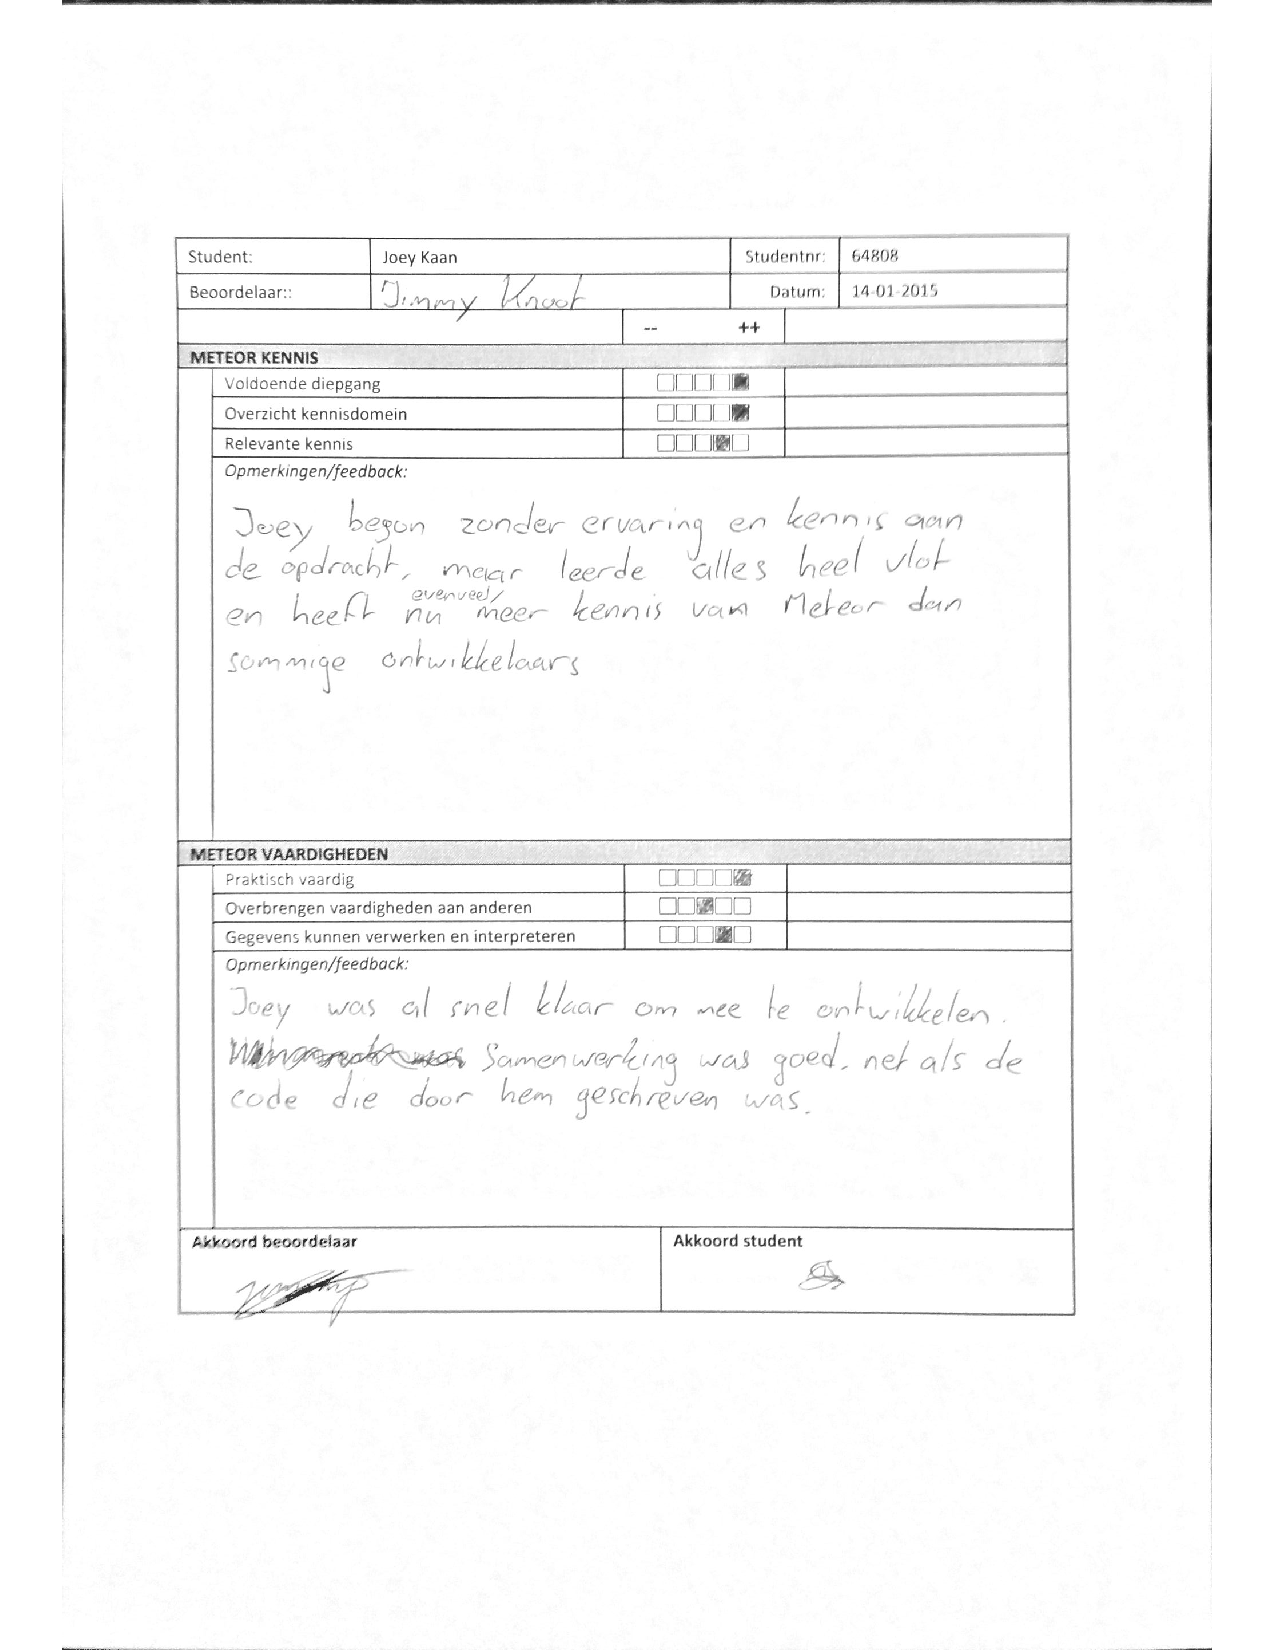
\includepdf[pages={1}, scale=0.65, pagecommand=\thispagestyle{fancy}]{attachments/beoordelingsformulier-meteor.pdf}
